\subsubsection{Company}
Meanwhile companies can also access the site to gain access to students. For example a recruiter from Netcraft, Sally, wishes to sign up in order to find talented students for placements.
  \paragraph{Sign up:}
    If Netcraft had not yet registered as a company, then the Sally must sign up on Netcrafts behalf with a clear and consise sign up page.

    \begin{figure}[H]\centering
    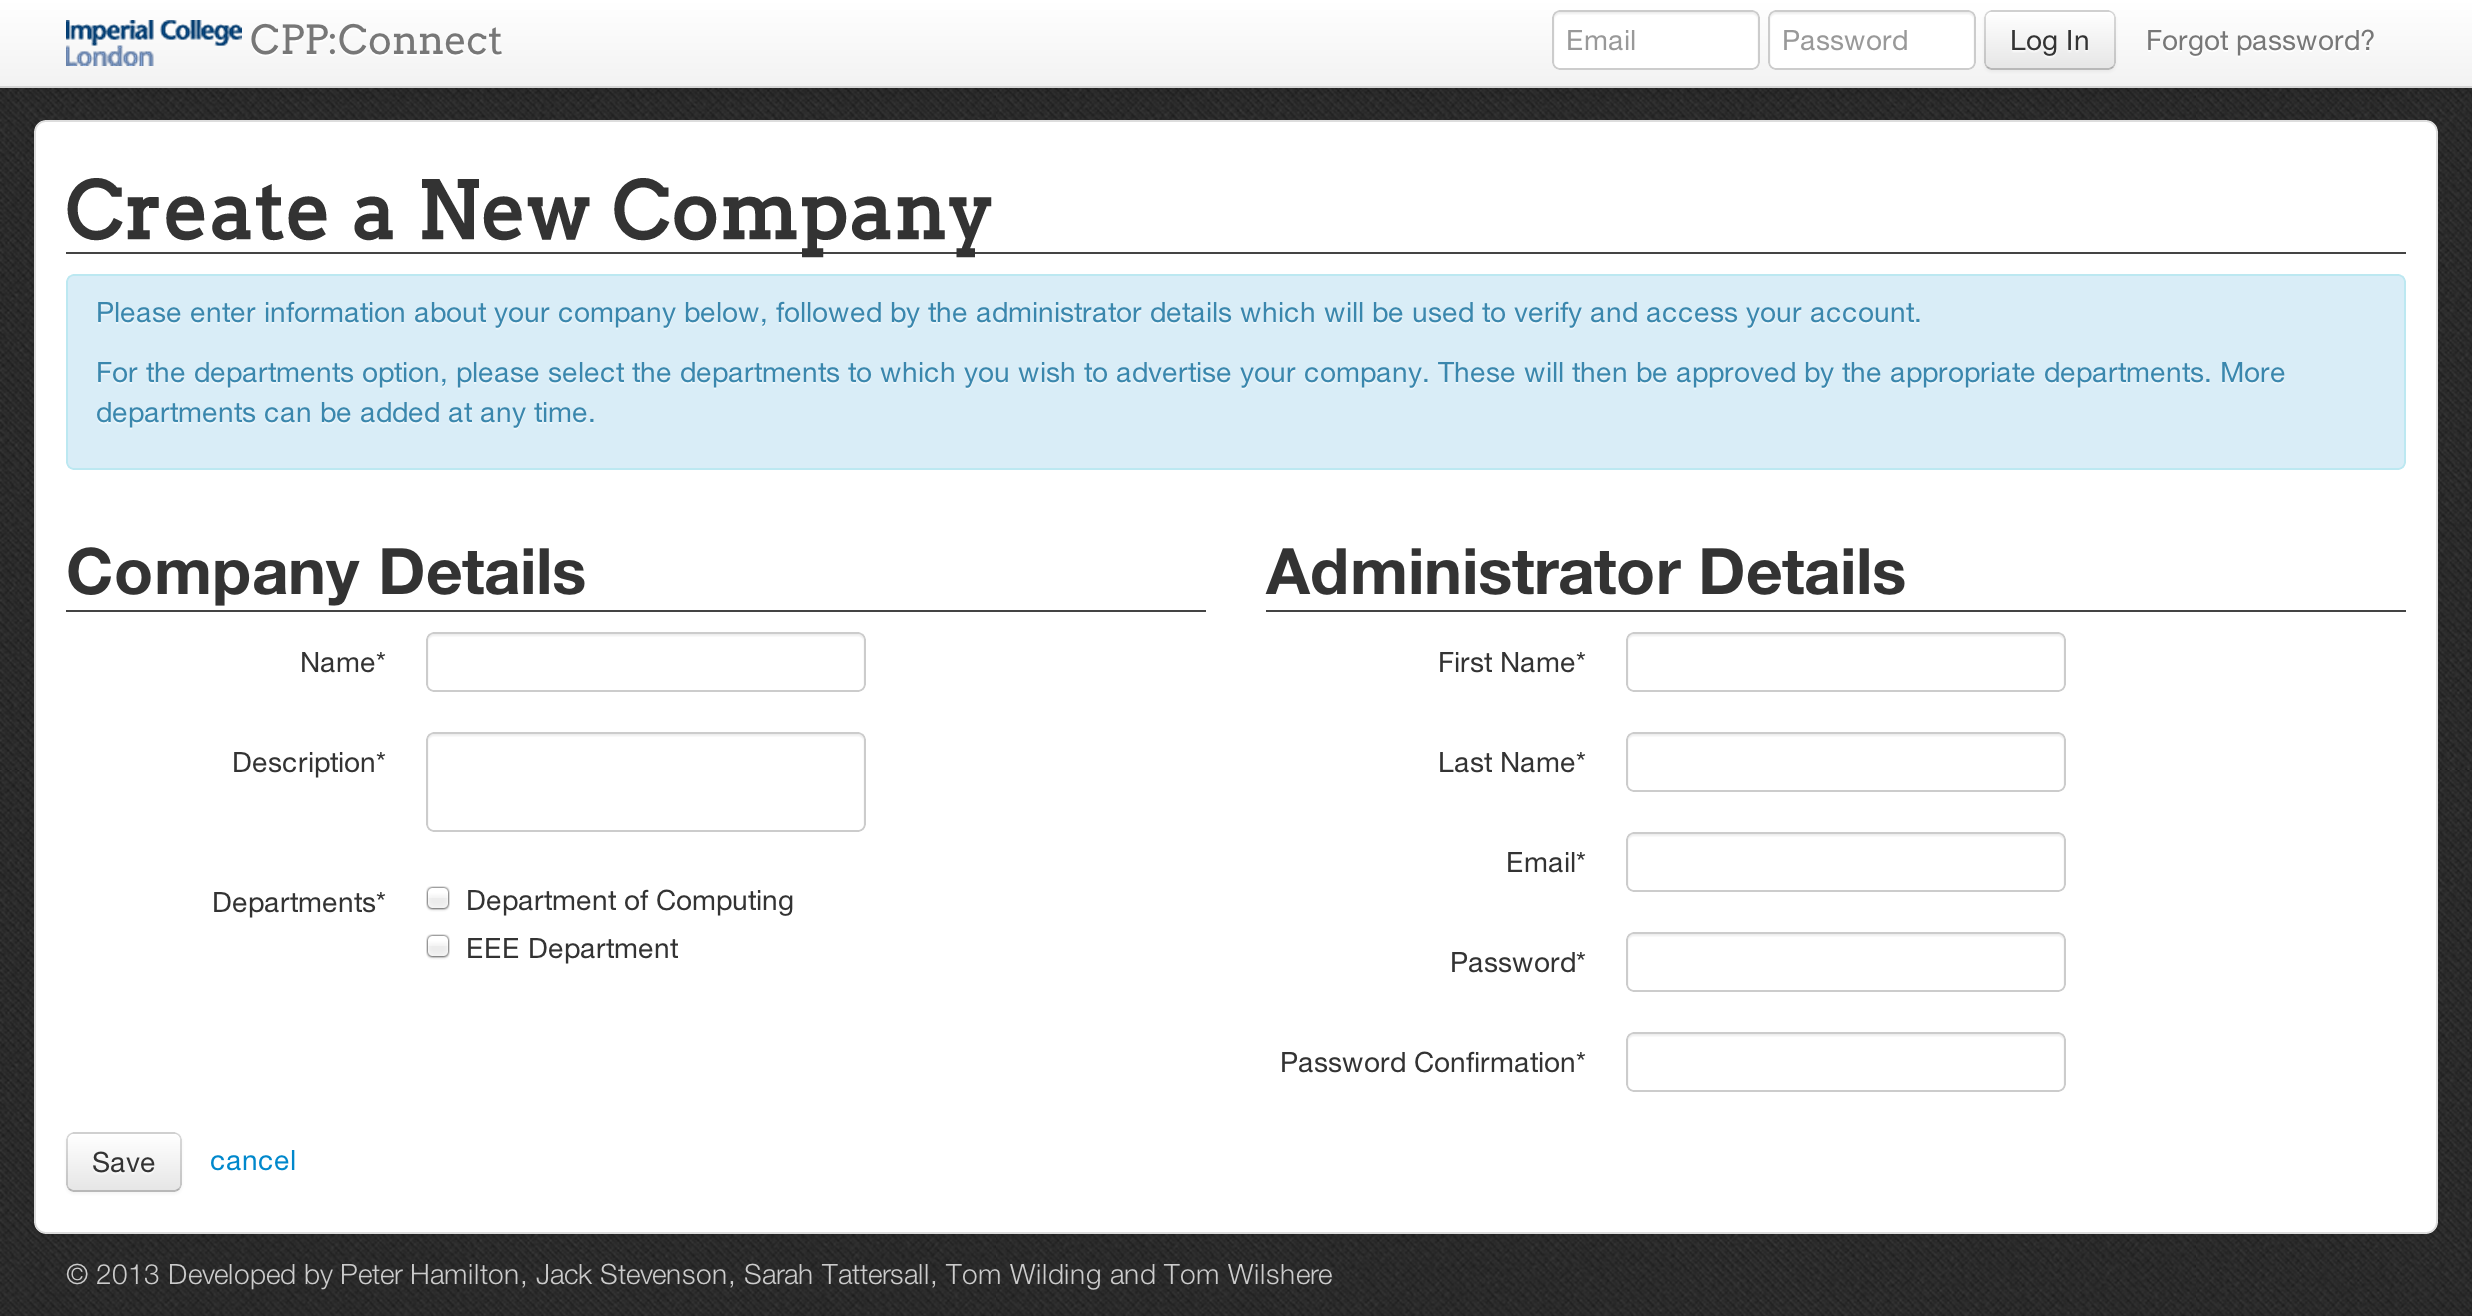
\includegraphics[scale=0.3]{images/user_experiences/company/company_signup}
    \caption{Company sign up page}
    \end{figure}

    On registering as a company we have taken the descion to not allow companies student access straight away. This is because our website is public and we may not want all companies to have student access. We envision that it might only ever be for the Corporate Partners, who invest money in our department - since we need to give them some incentive to pay!
    Whilst not having student access, they can still create events and placements and edit their company profile unless the admin decides to delete them. These events and placements will show up to the students.

    %TODO WRITE UP ABOUT ISSUE #241

    Since Netcraft actually already exists then Sally must request that another admininistrator adds her by having them sign in and clicking on the new administrator button. They can then fill in Sallys details for her to be able to log on at a later date.

  \paragraph{Dashboard}
    Once signed in Sally is relocated to her dashboard, which has the same useful tool tips and extra features as the student page.
    We decided that on login administrators have the right to delete other administrators but not themselves. This is to stop them accidentally deleting themselves and being locked out forever. It will also mean that if the company only has one administrator they cannot be deleted which would leave the company stagnent.

    On the dashboard Sally can see how many students has viewed Netcraft's profile, a low number is likely to indicate they are not advertising enough events and/or placements and so their prescence on the site is lacking. 

    %TODO: PRINT SCREEN WHEN MAILINGS FINISHED, THINK THAT A PRINT SCREEN IS ENOUGH TO EXPRESS WHAT SHE CAN DO?

  \paragraph{Contacts:}
    Sally decides that she wishes to be contacted by students regarding job oppourtunities so adds her details to the company contacts in the top right hand corner. This very nicely comes up with an in place form for Sally to fill out.
    She fills out her details and is pleased when her contact card appears at the top but just incase she wanted to move herself below anyone else she notices the useful tooltip that tells her contact cards are draggable.

    \begin{figure}[H]\centering
    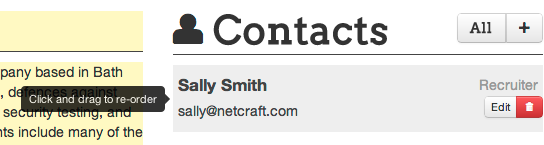
\includegraphics[scale=0.5]{images/user_experiences/company/netcraft_company_contact_tooltip}
    \caption{Tooltip for company contacts}
    \end{figure}
    Students viewing company pages can then email any of the contacts since they must disclose their email addresses.

  \paragraph{Events and Placements:}
    Sally decides that it might be a good idea to post that Netcraft is offering six month industrial placements and so clicks on the new placement button. 
    She receives important notices from the departments she's registered to that she reads and makes note of and then procedes to create the placement.
    %TODO PRINT SCREEN
    Similarly she can do the exact same thing with events.

    Sally then decides to look at an event that Netcraft is already advertising, as the event is coming up very soon she has the option to email the students more useful information, like how to get to Netcraft from the train station.
    This email will only be sent to receipients that are actually attending the event and must receive approval by a department admin before it is actually sent.

    %TODO CHECK THIS IMPLEMENTED
    [REMOVE THIS IF IT ISNT IMPLEMENTED] There is also a view all students button so that Sally can view who is planning to attend. We feel this feature might be more relevant after an event so that if a particular student stood out to her she can look them up online.
  
  \paragraph{Students:}
    After creating placements and events Sally decides she wants to browse students to find exceptional candidates she can contact herself. She clicks on students on the navigation bar and is greeted by a list of students. Note that any students who have decided to blacklist Netcraft will never appear in this list, nor will deactivated students.
    Since she knows Netcraft will be recruiting for Perl developers, she specifically types Perl into the skills filter
    and filters the list down to the students who have it as a skill.
    %TODO print screen
    She can then browse their profiles, which is a reduced version of the student view lacking the events and placement partial views since they are not relevant to her. Since Jack has listed Perl as a skill his profile appears on the list.

    %REDO THIS WHEN IT HAS MAIL TO
    \begin{figure}[H]\centering
    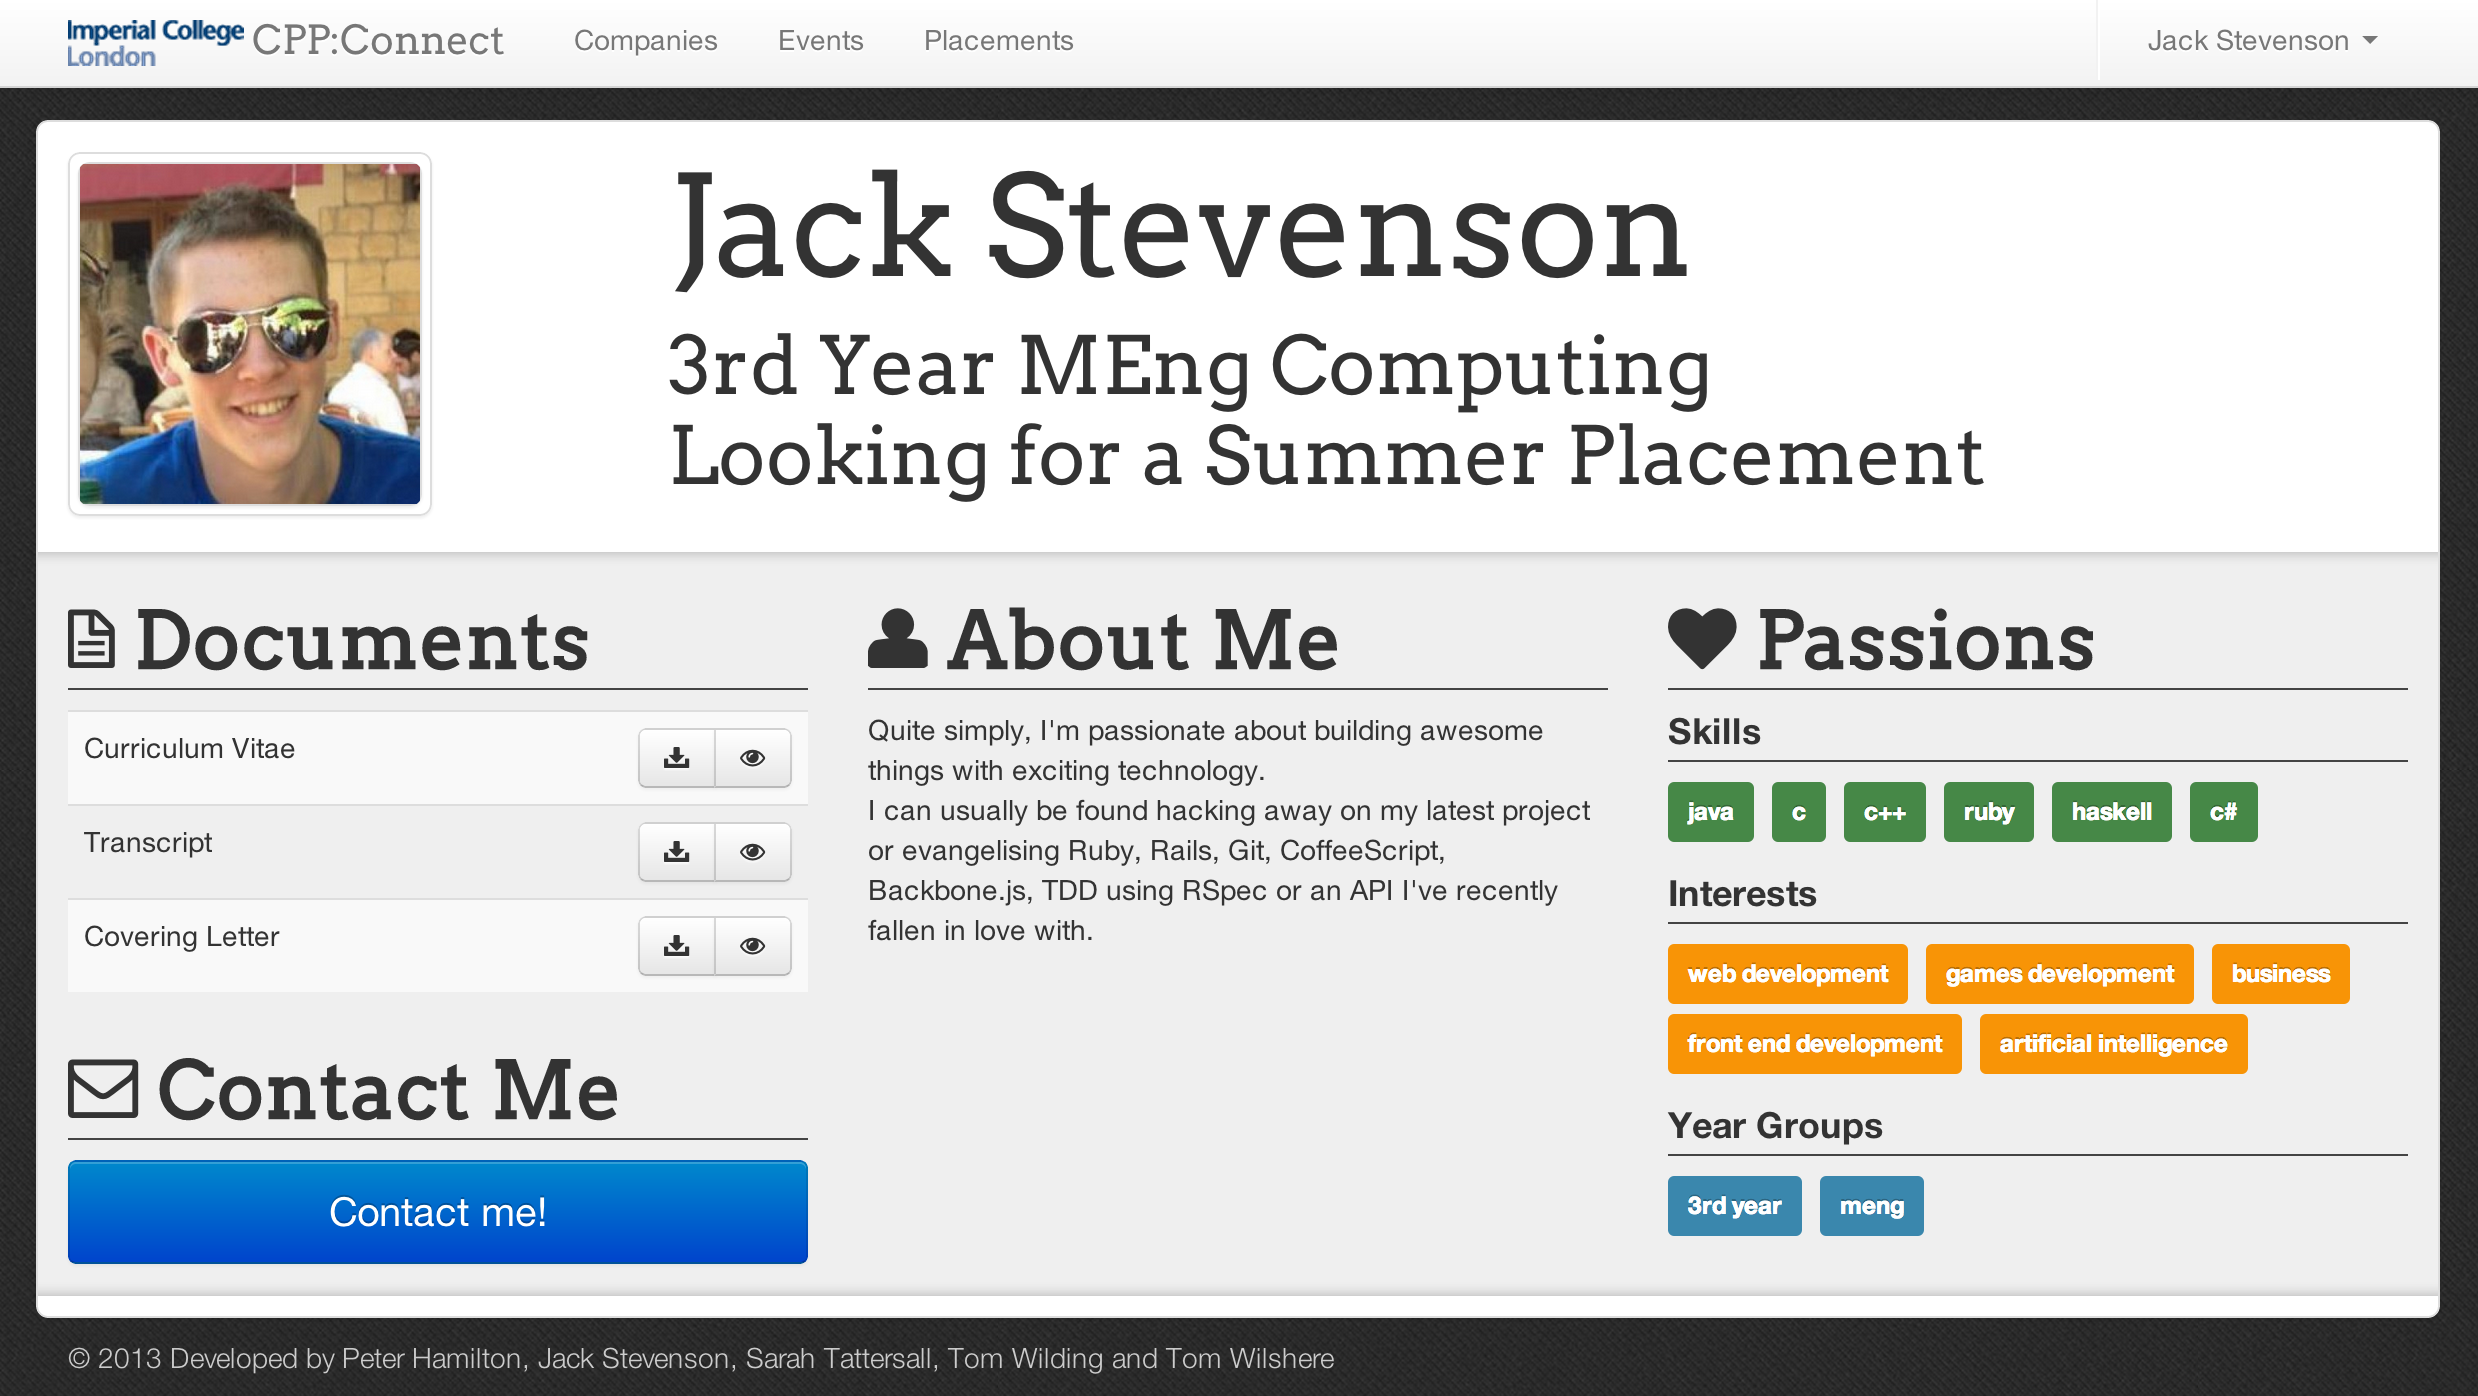
\includegraphics[scale=0.3]{images/user_experiences/company/jack_profile}
    \caption{Company view of student profile}
    \end{figure}

    Liking what she see's Sally can then choose to download Jack's CV to her computer or view it online with the preview icon button and after reading Jacks CV Sally then chooses to invite Jack to interview, by clicking on the `contact me' button which we have made large to avoid being unnoticed. She then sends an email from her account to his address which he can reply to if he wants. 

    If a student gets fed up with receiving personal emails from Netcraft, their blocking feature easily ensures Netcraft can never contact them again.

  \paragraph{Emails:}
    Being a member of the Corporate Partnership Program entitles Netcraft to be able to contact a departments students via email. Sally can create emails to inform students of exciting scholarships Netcraft are offering, or news about the company. The great thing about our email client is that it supports HTML, so company styles can be used when sending emails through our system. Many companies use HTML emails with rich content when emailing students at the moment so this will allow this practice to continue, and indeed encourages companies to spend more time making their emails look enticing.

    After writing any emails she must wait for them to be approved by an admin. 

    We have chosen for emails to be approved by an admin to avoid companies being able to spam students and hope that the need for admin approval encourages them to write detailed informative emails that are of an appropriate content for students. If it is not deemed applicable enough the admin can send the email back to the company for modifying with the reason, or reject it all together.
    We do not at current require approval for personal emails to students as this is deemed too much work for a CPP administrator.  


    %%%%%%%%%%%%%%%%%%%%%%%%%%%% TODO %%%%%%%%%%%%%%%%%%%%%%%%%%%%%
    % * Companies requesting permissions for students, perhaps Sally wants Maths students?
    % * Print screens
    % * Describe a little more about the emails
    %%%%%%%%%%%%%%%%%%%%%%%%%%%%%%%%%%%%%%%%%%%%%%%%%%%%%%%%%%%%%%%
